% ===========================================================================
\section{Timing, camino crítico y frecuencia}
\label{sec:timing}

Todas las mediciones son post-implementación (\texttt{Design State: Routed}) con Vivado~2024.2,
tomadas con \repo{scripts/timing.tcl} y \repo{scripts/barrido.tcl}. Los reportes y las capturas
están en \repo{docs/timing/}.

\subsection{Cómo se llegó a la frecuencia final}

\begin{enumerate}[nosep]
  \item \textbf{\qty{100}{\mega\hertz} sin Clock Wizard (I-49).} Ya la estimación post-síntesis
        no cerraba (WNS $-5{,}227$~ns): el camino de la redirección de un salto no entraba en
        \qty{10}{\nano\second}.
  \item \textbf{\qty{65}{\mega\hertz} con el Clock Wizard (\decision{042}).} Para tener la placa
        funcionando mientras tanto.
  \item \textbf{Comparador de igualdad (I-56, \decision{044}).} Se midió el camino crítico y se
        sacó la ALU de la decisión del salto: el slack a \qty{65}{\mega\hertz} pasó de
        $+0{,}435$ a $+1{,}418$~ns, sin cambiar ciclos, modelo ni resultados esperados.
  \item \textbf{Barrido de 65 a \qty{100}{\mega\hertz} (I-57, \decision{045}).} Se implementó el
        diseño desde cero en 16 frecuencias y se eligió la máxima que cumple timing:
        \textbf{\qty{92}{\mega\hertz}}.
\end{enumerate}

\subsection{Camino crítico antes y después del comparador}

La \decision{012} supuso que el camino crítico sería la decisión de un salto que compara un dato
recién cargado: después del stall, el dato llega por forwarding desde MEM/WB, el salto se decide en
EX y en el mismo ciclo redirige el PC y anula IF/ID e ID/EX. La medición a \qty{65}{\mega\hertz}
lo confirmó, con una corrección: el tramo largo no era la resta sino el \textbf{desplazador} y el
mux de resultado de la ALU, porque \texttt{zero} salía del resultado ya multiplexado de las diez
operaciones.

\begin{center}
\small
\begin{tabular}{@{}l l r r@{}}
  \toprule
  \textbf{Tramo} & \textbf{Etapa} & \textbf{Base} & \textbf{Comparador} \\
  \midrule
  \texttt{dmem\_bram} \emph{clock-to-out} y ruteo    & MEM $\to$ WB & 3,537 & 3,885 \\
  Extensión del load y mux de \texttt{wb\_data}       & WB & 1,608 & 2,642 \\
  Mux de forwarding                                    & EX & 0,964 & 0,846 \\
  Mux de \texttt{alu\_b}, ALU y \texttt{zero}          & EX & 6,860 & \textemdash \\
  Comparador \texttt{rs1\_val == rs2\_val}             & EX & \textemdash & 2,681 \\
  \texttt{taken} y \texttt{redirect}                   & EX & 0,570 & 1,081 \\
  Unidad de riesgos (flush o enable)                   & ID / IF & 0,675 & 2,016 \\
  \midrule
  \textbf{Total de datos (ns)}                         & & \textbf{14,212} & \textbf{13,151} \\
  Slack a \qty{65}{\mega\hertz} (ns)                   & & $+0{,}435$ & $+1{,}418$ \\
  \bottomrule
\end{tabular}
\end{center}

El comparador reemplaza 6,86~ns por 2,68~ns. La mejora neta del retardo es menor (1,06~ns) porque
la colocación cambió de una corrida a otra y el WB salió más largo: entre el 60 y el 70\,\% del
camino es ruteo. Por la misma razón la estimación post-síntesis no sirve para decidir.

\begin{figure}[H]
  \centering
  \begin{subfigure}{0.49\linewidth}
    \centering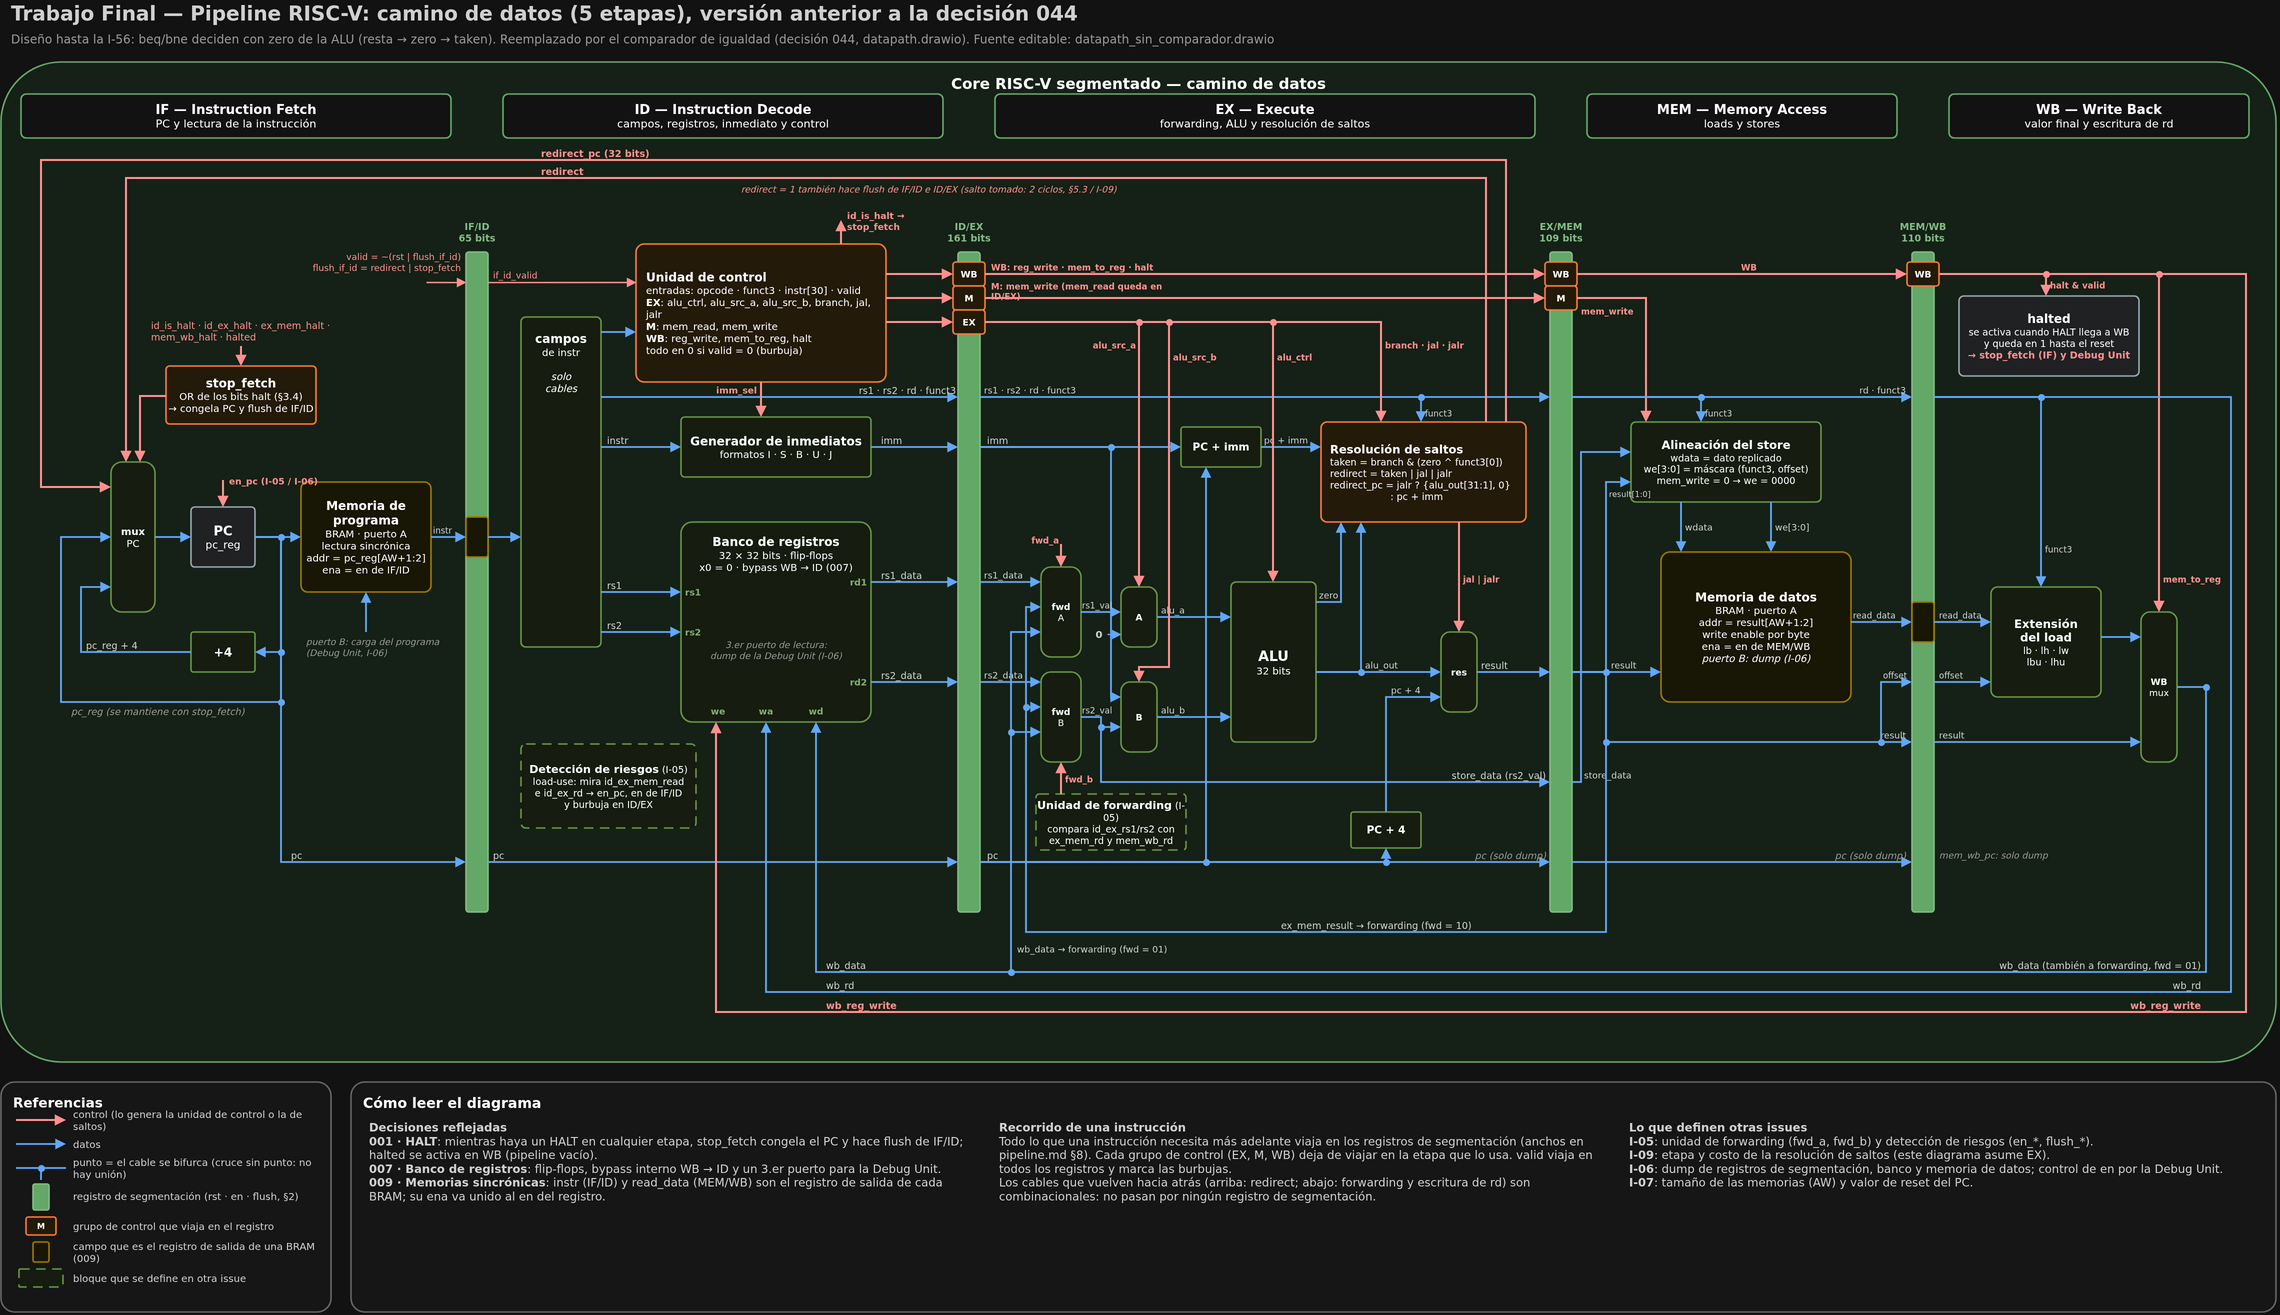
\includegraphics[width=\linewidth]{datapath_sin_comparador.png}
    \caption{Base: el salto decide con \texttt{zero} de la ALU.}
  \end{subfigure}\hfill
  \begin{subfigure}{0.49\linewidth}
    \centering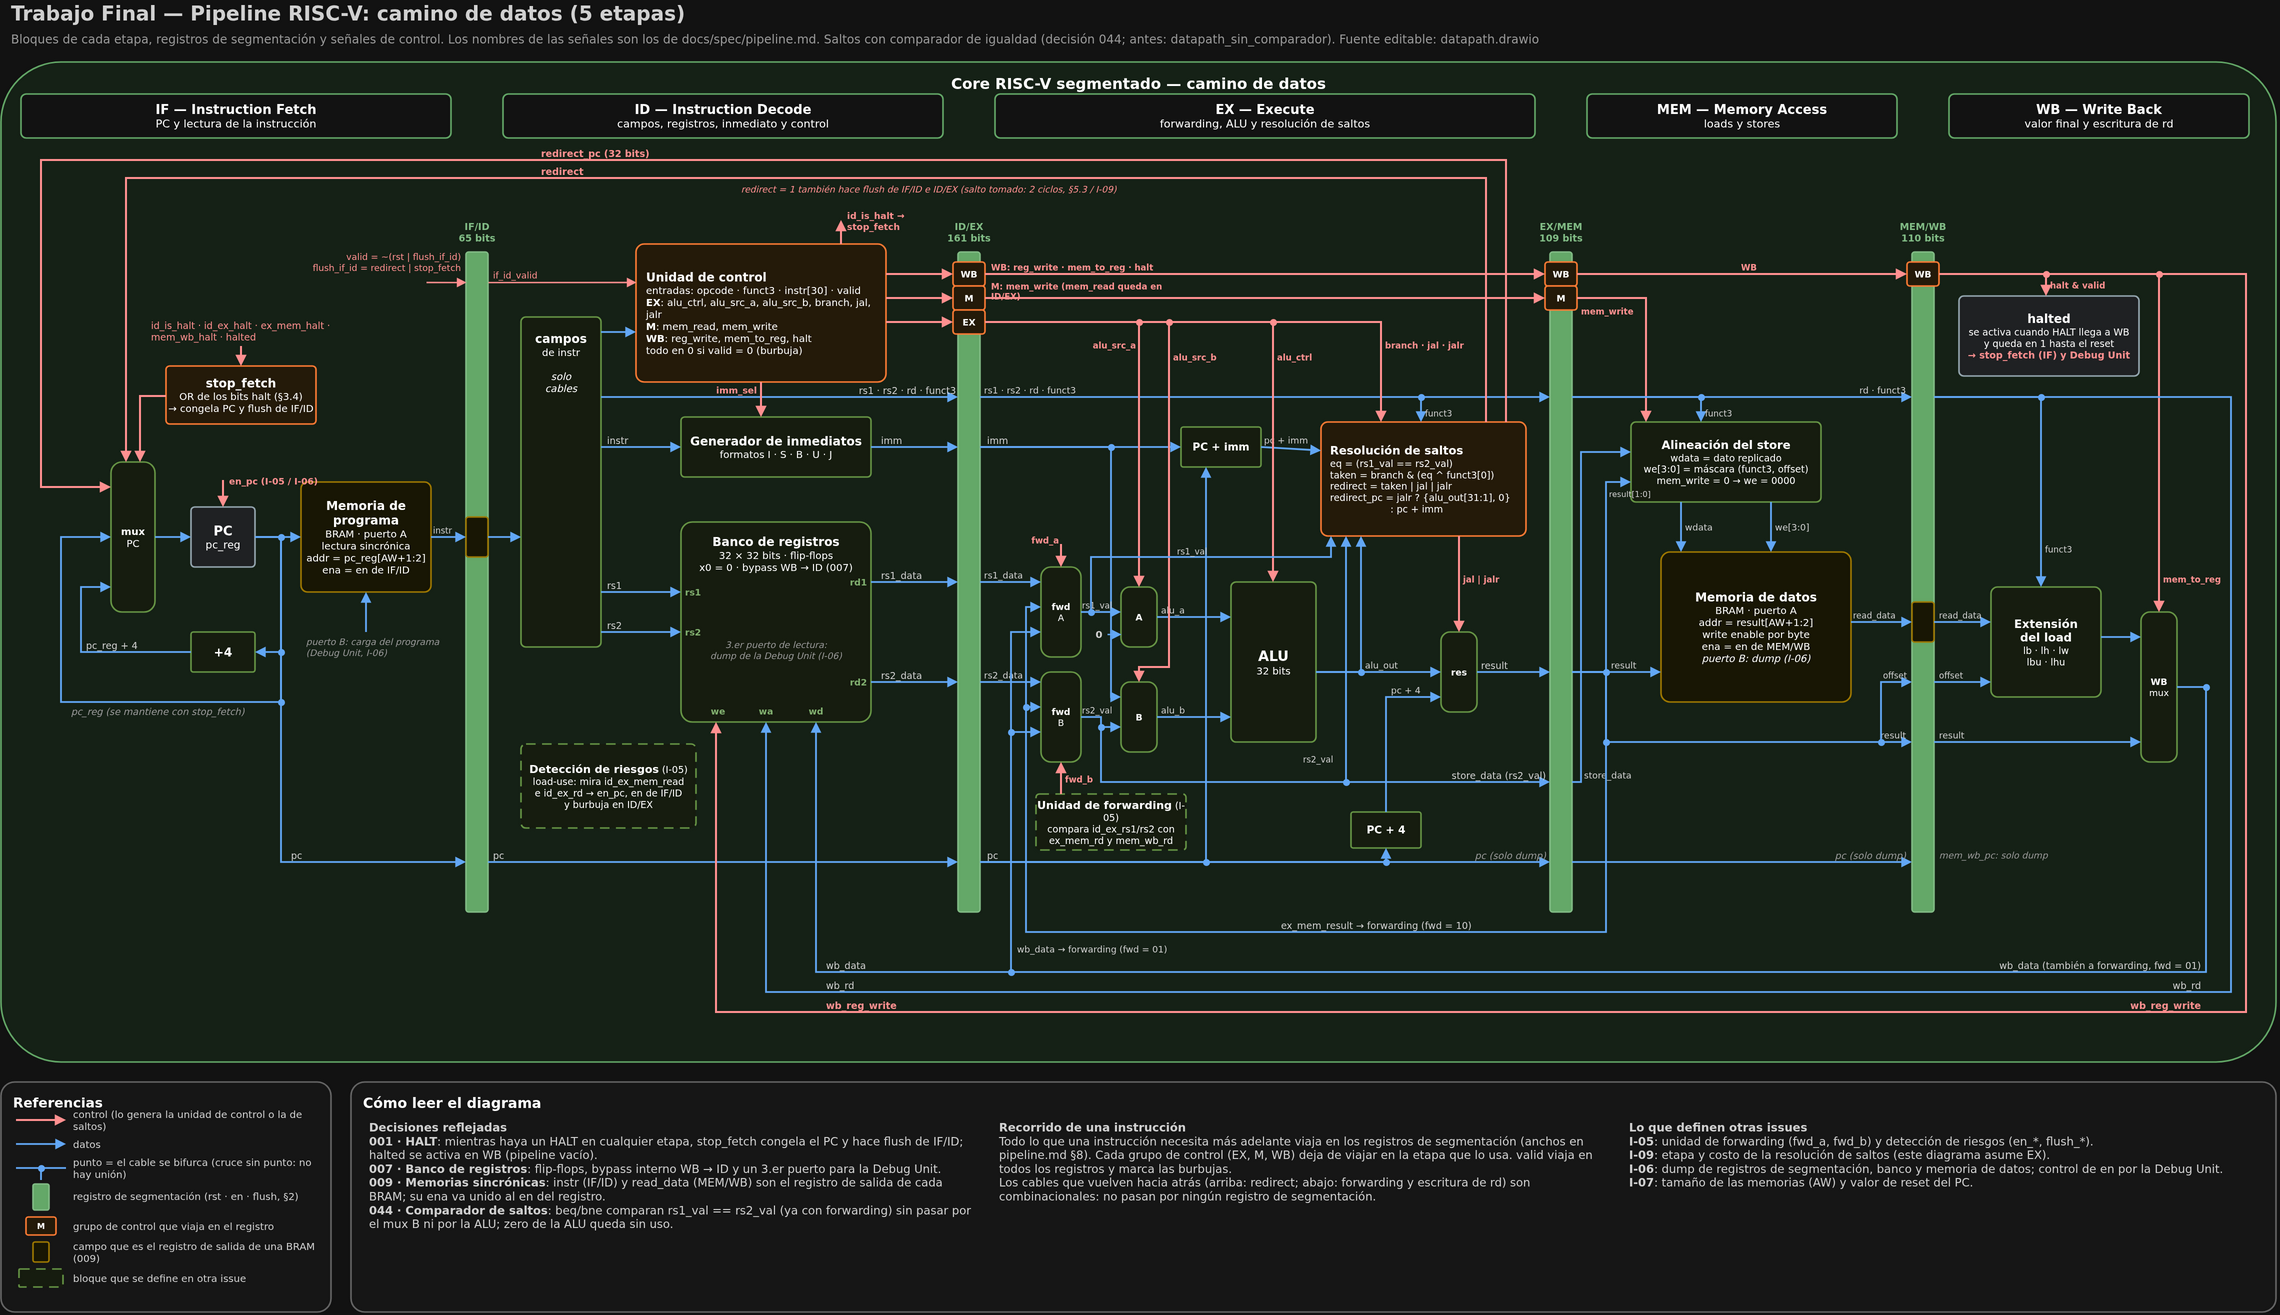
\includegraphics[width=\linewidth]{datapath.png}
    \caption{Final: comparador de igualdad (\decision{044}).}
  \end{subfigure}
  \caption{\textbf{Camino de datos antes y después del comparador.} El cambio está en EX: la
  decisión del salto deja de pasar por el mux del operando~B y la ALU.}
  \label{fig:comparador}
\end{figure}

\subsection{Barrido de frecuencias}

\begin{center}
\small
\begin{tabular}{@{}r r r r r r@{}}
  \toprule
  \textbf{MHz} & \textbf{WNS (ns)} & \textbf{TNS (ns)} & \textbf{Fallan} & \textbf{WHS (ns)} & \textbf{Peor camino (ns)} \\
  \midrule
  65  & $+1{,}418$ & 0 & 0 & $+0{,}066$ & 13,151 \\
  70  & $+1{,}111$ & 0 & 0 & $+0{,}037$ & 12,991 \\
  74  & $+1{,}078$ & 0 & 0 & $+0{,}037$ & 11,498 \\
  76  & $+0{,}229$ & 0 & 0 & $+0{,}045$ & 12,438 \\
  80  & $+0{,}412$ & 0 & 0 & $+0{,}046$ & 11,711 \\
  86  & $+0{,}409$ & 0 & 0 & $+0{,}051$ & 11,031 \\
  90  & $+0{,}288$ & 0 & 0 & $+0{,}098$ & 10,650 \\
  \textbf{92} & $\mathbf{+0{,}026}$ & 0 & 0 & $+0{,}037$ & 10,117 \\
  95  & $-0{,}449$ & $-5{,}893$ & 42 & $+0{,}037$ & 10,720 \\
  100 & $-0{,}714$ & $-30{,}251$ & 122 & $+0{,}075$ & 10,598 \\
  \bottomrule
\end{tabular}
\end{center}

La tabla es un extracto de las 16 frecuencias (\repo{docs/timing/i57_barrido/barrido.csv}). Muestra
tres cosas:

\begin{itemize}[nosep]
  \item \textbf{La cota de la medición a \qty{65}{\mega\hertz} era pesimista.} Suponía el mismo
        ruteo con otro reloj ($\approx$\qty{71,6}{\mega\hertz}). Con un reloj más exigente, la
        colocación y el ruteo guiados por timing acortan el camino: el retardo de datos baja de
        13,15 a 10,12~ns.
  \item \textbf{El resultado no es monótono.} De 76 a \qty{90}{\mega\hertz} el WNS sube y baja,
        y en algunas frecuencias el Clock Wizard elige otros divisores con menos jitter.
  \item \textbf{El flujo es determinista.} \qty{92}{\mega\hertz} se implementó tres veces (barrido,
        \repo{timing.tcl} y la GUI) con el mismo $+0{,}026$~ns.
\end{itemize}

Se eligió \textbf{\qty{92}{\mega\hertz}}, la máxima que cierra: el análisis estático ya usa el peor
caso de proceso, tensión y temperatura, así que con WNS $\geq 0$ el diseño funciona en la placa
(\decision{045}). El MMCM da exactamente $100 \times 48{,}875 / (5 \times 10{,}625) =
92{,}000$~MHz.

\subsection{Diseño final a \qty{92}{\mega\hertz}}

\begin{center}
\small
\begin{tabular}{@{}p{3.6cm} p{12cm}@{}}
  \toprule
  Período                 & 10,870~ns \\
  WNS / TNS (setup)       & $+0{,}026$~ns / 0, 0 de 5360 endpoints fallan \\
  WHS / THS (hold)        & $+0{,}037$~ns / 0 \\
  Peor camino             & \texttt{dmem\_bram} $\to$ WB $\to$ forwarding $\to$ comparador $\to$ \texttt{redirect} $\to$ flush de ID/EX; 10,117~ns, 9 niveles \\
  LUT / LUTRAM / FF       & 2907 (14\,\%) / 22 / 1884 (5\,\%) \\
  BRAM / MMCM / IO        & 2 RAMB36 (4\,\%) / 1 / 20 \\
  Consumo estimado        & 0,200~W (0,128 dinámico, de los que el MMCM es 0,120) \\
  UART                    & $\mathrm{DVSR} = 50$, 115\,000 baudios (\qty{-0,17}{\percent}) \\
  \bottomrule
\end{tabular}
\end{center}

A \qty{92}{\mega\hertz} varias etapas quedan en el límite, y todas empiezan en el
\emph{clock-to-out} de la BRAM de datos: EX/MEM a $+0{,}114$~ns (forwarding $\to$ ALU),
\texttt{pc\_reg} a $+0{,}171$~ns, el \emph{enable} de la memoria de programa a $+0{,}428$~ns. No hay
un único camino que, acortado, permita subir mucho más; por eso a \qty{95}{\mega\hertz} fallan 42
endpoints con destinos distintos.

\begin{figure}[H]
  \centering
  \begin{subfigure}{0.49\linewidth}
    \centering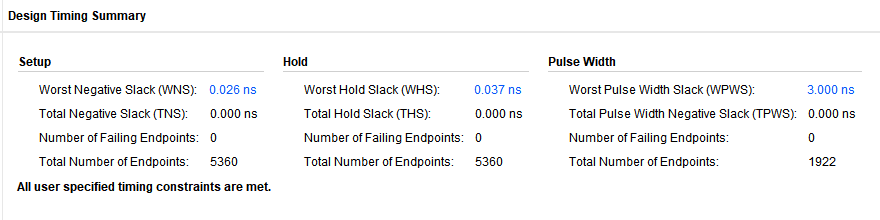
\includegraphics[width=\linewidth]{i57_92mhz/vivado_timing.png}
    \caption{\emph{Design Timing Summary} post-implementación.}
  \end{subfigure}\hfill
  \begin{subfigure}{0.49\linewidth}
    \centering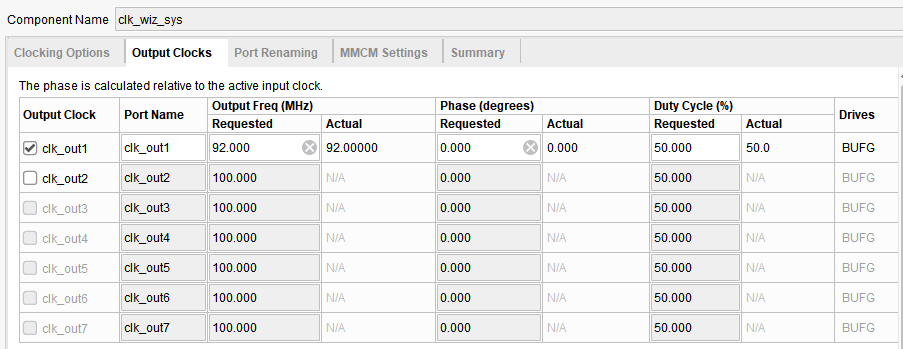
\includegraphics[width=\linewidth]{i57_92mhz/vivado_clk_wiz_salidas.png}
    \caption{Clocking Wizard: \qty{92,000}{\mega\hertz}.}
  \end{subfigure}
  \caption{\textbf{Implementación a \qty{92}{\mega\hertz} en Vivado.} Más capturas (MMCM, relojes,
  utilización, consumo y DRC) en \repo{docs/timing/i57_92mhz/}.}
  \label{fig:vivado92}
\end{figure}

\paragraph{Lo que no se aplicó.} El registro de salida de las BRAM sacaría su
\emph{clock-to-out} del camino crítico, y registrar \texttt{redirect} cortaría el camino del salto.
Las dos opciones suman ciclos (un load-use pasaría a costar 2 stalls y un salto tomado 3 ciclos) y
cambian el modelo y todos los \texttt{.exp}, a cambio de una frecuencia mayor. No se aplicaron: la
consigna evalúa la frecuencia y el análisis del camino, y con el comparador el diseño ya cumple
con margen positivo.

\subsection{Skew}
\label{sec:skew}

El diseño tiene un solo reloj (\texttt{clk\_out1\_clk\_wiz\_sys}) que sale del MMCM por un BUFG
hacia todos los elementos sincrónicos; el otro BUFG es la realimentación del MMCM. No hay
\texttt{BUFGCE}, divisores ni relojes generados con lógica.

\begin{center}
\small
\begin{tabular}{@{}p{5.4cm} p{10.2cm}@{}}
  \toprule
  \multicolumn{2}{@{}l}{\textbf{A \qty{92}{\mega\hertz}}} \\
  \midrule
  Skew del camino crítico de setup & $-0{,}073$~ns (0,7\,\% del período) \\
  Incertidumbre del reloj (jitter) & 0,129~ns \\
  Peores de setup por etapa        & de $-0{,}116$ a $+0{,}029$~ns \\
  Peores de hold por etapa         & de 0 a $+0{,}265$~ns (el mayor, de MEM/WB al banco, con slack $+0{,}455$~ns) \\
  \bottomrule
\end{tabular}
\end{center}

\begin{itemize}[nosep]
  \item \textbf{Setup}: un skew negativo (el reloj llega antes al destino) le quita tiempo al
        dato. Son 73~ps de 10,87~ns: pesa más el jitter, y ninguno de los dos limita la
        frecuencia. La limita el camino de datos.
  \item \textbf{Hold}: el peligro es el skew positivo, porque el dato nuevo puede pisar al viejo
        antes de capturarse. Todos los caminos tienen slack positivo. El hold no depende de la
        frecuencia: un WHS negativo no se arreglaría bajando el reloj.
  \item \textbf{Por qué es chico}: el árbol global de la FPGA está balanceado y el MMCM compensa el
        retardo de inserción con su realimentación (por eso Vivado muestra retardos de reloj
        negativos). Un reloj gateado para el paso a paso saldría por ruteo común, con skew del orden
        de los nanosegundos y violaciones de hold que Vivado no puede corregir. Es la razón de la
        \decision{018}.
\end{itemize}
